\part{Non-singular case}

\section{The model}

    We consider an $\mN=2$ gauge theory with gauge group $\SU(N_c)$ and with $N_f$ hypermultiplets, i.e. $\mN=2$ SQCD with $N_c$ colors and $N_f$ flavors. Recall the following decomposition of $\mN=2$ superfields in terms of $\mN=1$ superfields:
    \begin{align}
        [\mN=2 \text{ vector multiplet}] &: V=(\lambda_\alpha,A_\mu,D)\oplus \Phi=(\phi,\psi_\alpha,F)\\
        [\mN=2 \text{ hypermultiplet}] &: Q=(H_1,\psi_{1\alpha},F_1) \oplus \tilde{Q}=(\bar{H}_2,\bar{\psi}_{2\dalpha},\bar{F}_2)
    \end{align}
    where $V$ is a vector superfield and $\Phi,H_1,H_2$ are chiral superfields. We denote by $\W_\alpha$ the chiral superfield strength associated to $V$. We have
    \begin{itemize}
        \item $V$ is a vector superfield transforming in the adjoint of $\SU(N_c)$. It belongs to $\mathfrak{su}(N_c)$ and his components are denoted by $V^a_b$ with $a,b=1,\dots,N_c$.
        \item $\Phi$ is a chiral superfield transforming in the adjoint of $\SU(N_c)$. It belongs to $\mathfrak{su}(N_c)$ and his components are denoted by $\Phi^a_b$ with $a,b=1,\dots,N_c$.
        \item $Q^i$ ($i=1,\dots,N_f$) are $N_f$ chiral superfields transforming in the $\boldsymbol{N_C}$ of $\SU(N_c)$ and in the $\boldsymbol{N_f}$ of the global group $\SU(N_f)$. It has $N_c$ components, denoted by $Q^i_a$.
        \item $\tilde{Q}_i$ are $N_f$ chiral superfields transforming in the $\bar{\boldsymbol{N_C}}$ of $\SU(N_c)$ and in the $\bar{\boldsymbol{N_f}}$ of the global group $\SU(N_f)$. It has $N_c$ components, denoted by $\tilde{Q}^a_i$.
    \end{itemize}
    $Q$ and $\tilde{Q}$ are called the \emph{quark superfields}, $H_1$ and $H_2$ the \emph{squarks} and $\phi$ the \emph{adjoint-scalar}. The lagrangian reads
    \begin{equation}
        \L^{\mN=2}_{\text{SYM}} = \frac{1}{4\pi}\Im\left[\tau\int\d^2\theta\d^2\bar{\theta}\tr\left(\Phi^\dagger e^V\Phi + Q^\dagger_i e^V Q^i + \tilde{Q}^{\dagger i}e^V \tilde{Q}_i\right)+\tau\int\d^2\theta\left(\frac{1}{2}\tr(\W^\alpha\W_\alpha)+W(\phi,H_1,H_2)\right)\right]\label{eq:lag}
    \end{equation}
    where $W(H_1,H_2)$ is the $\mN=2$ superpotential
    \begin{align}
        W(\phi,H_1,H_2) &= \sqrt{2}H_1\phi H_2 + mH_1H_2 \\
        &= \sqrt{2}(H_2)^a_i\phi^b_a (H_1)^i_b + \sqrt{2}m^i_j(H_2)^a_i(H_1)^j_a
    \end{align}
    and $\tau$ is the complexified gauge coupling
    \begin{equation}
        \tau=\frac{\theta}{\pi}+i\frac{8\pi}{g^2}.
    \end{equation}
    The matrix $m$ has to satisfy
    \begin{equation}
        [m,m^\dagger]=0
    \end{equation}
    in order to preserve $\mN=2$ supersymmetry, it is called the \emph{quark mass matrix}. This matrix can be diagonalized by an $\SU(N_f)$ transformation, i.e. a flavor rotation, to become
    \begin{equation}
        m=\text{diag}(m_1,\dots,m_{N_f}).
    \end{equation}

    Classically and with $m=0$ the global symmetry should be $\SU(N_f)\times\U(1)_B\times\U(2)_R$. The mass terms and instanton corrections breaks $\U(1)_R$ of the $R$-symmetry, leaving the compact component $\SU(2)_R$ unbroken. The lagrangian should be invariant under the latter, it is a necessary and sufficient condition to have $\mN=2$ supersymmetry. Under the unbroken $\SU(2)_R$, the bosonic fields of the vector multiplet, i.e. $A_\mu,\phi,D,F$ are singlets butthe fermions form a doublet $(\lambda_\alpha,\psi_\alpha)$. Similarly, for the hypermultiplets, the fermions $\psi_{1\alpha},\bar{\psi}_{2\dalpha}$ are singlets while their scalar superpartners for a doublet $(H_1,\bar{H_2})$. The $\SU(2)_R$ symmetry cannot be made manifest in terms of $\mN=1$ sueprfields but the symmetry $\U(1)_J\subset\SU(2)_R$ is manifest in \eqref{eq:lag}.
    
    The selection rules resulting from the breaking of the classical symmetries by mass terms and instanton corrections can be describe bt assigning symmetry transformation properties to the corresponding parameters in the action. In particular, the quark mass matrix $m$ can be decomposed into a trace part $m_S$ that transforms as a singlet under $\SU(N_f)$ and a traceless part $m_A$ that transforms in the adjoint of $\SU(N_f)$. We summarize all the representations in which the fields and the parameters transform transform in table \ref{table:fieldrepr}.

    \begin{table}[H]
        \centering
        $
        \begin{array}{c|ccccc}
            & \SU(N_c) & \SU(N_f) & \U(1)_B & \U(1)_R & \U(1)_J \\ \hline
            \Phi & \textbf{adj} & \boldsymbol{1} & 0 & 2 & 0 \\
            Q & \boldsymbol{N_c} & \boldsymbol{N_f} & 1 & 0 & 1 \\
            \tilde{Q} & \bar{\boldsymbol{N_c}} & \bar{\boldsymbol{N_f}} & -1 & 0 & 1 \\
            m_A & \boldsymbol{1} & \textbf{adj} & 0 & 2 & 0 \\
            m_S & \boldsymbol{1} & \boldsymbol{1} & 0 & 2 & 0 \\
            \Lambda^{2N_c-N_f} & \boldsymbol{1} & \boldsymbol{1} & 0 & 2(2N_c-N_f) & 0
        \end{array}
        $
        \caption{Field representations.}
        \label{table:fieldrepr}
    \end{table}

    For $\mN=2$ theories, the $\beta$ function is exact at $1$-loop and $\beta_{1\text{-loop}}\propto 2N_c-N_f$. If if $N_f<2N_c$, the $\beta$-function is negative. The theory is asymptotically free and it generates a strong-coupling scale $\Lambda$. The instanton factor is proportional to $\Lambda^{2N_c-N_f}$ and the $\U(1)_R$ symmetry is anomalous. It is broken down to a discrete $\Z_{2N_f-N_c}$ symmetry. For $N_f=2N_c$, the theory is scale invariant and $\U(1)_R$ symmetry is not anomalous. No strong-coupling scale is generated and the theory is described in terms of its bare couplings.

    $D,F,F_1$ and $F_2$ are auxiliary fields and their equations of motion are:
    \begin{align}
        F^a_b &= \pdv{W}{\phi^b_a} = \sqrt{2}(H_2)^a_i (H_1)^i_b\\
        (F_1)^a_i &= \pdv{W}{(H_{1})^i_a} = \sqrt{2}(H_2)^b_i\phi^a_b + \sqrt{2}m^j_i(H_2)^a_j,\\
        (F_2)^i_a &= \pdv{W}{(H_{2})^a_i} = \sqrt{2}\phi^b_a (H_1)^i_b + \sqrt{2}m^i_j(H_1)^j_a,\\
        D^A &= -[\phi,\phi^\dagger]^A + \bar{H}_1T^AH_1-\bar{H}_2T^AH_2
    \end{align}
    where $T^A$ are the generators of $\SU(N_f)$ and $A=1,\dots,N^2_f-1$. Note that we can also integrate out the auxiliary fields $F_1$ and $F_2$ to recast the scalar potential for the hypermultiplets as a D-term contribution. The potential reads
    \begin{align}
        V(\phi,H_1,H_2) &= \frac{1}{2}\tr(D^AD_A)+\bar{F}F+\bar{F_1}F_1+\bar{F_2}F_2\\
        &= \frac{1}{2}\tr([\phi,\phi^\dagger]^2)+\frac{1}{2}\abs{\bar{H}_1T^AH_1-\bar{H}_2T^AH_2}^2\\
        &\qquad+2\abs{(H_2)^b_i\phi^a_b+m^j_i(H_2)^a_j}^2+2\abs{\phi^b_a (H_1)^i_b+m^i_j(H_1)^j_a}^2
    \end{align}

\section{Classical moduli space}

    The D-term and F-term equations are
    \begin{figure}[H]
        \centering
        $
        \begin{array}{|cc|}
            \hline
            & \\
            D:& \begin{cases}
                \hspace{3.1cm}[\phi,\phi^\dagger]  &= 0 \\
                (H_1)^i_a(H^\dagger_1)^b_i-(H^\dagger_2)^i_a(H_2)^b_i &= \nu\delta^a_b
            \end{cases}\\
        & \\
        F:&
        \begin{cases}
            \hspace{1.3cm}(H_1)^i_a(H_2)^b_i &= \rho\delta^b_a \\
            (H_1)^j_am^i_j+\phi^b_a(H_1)^i_b &= 0 \\
            m^i_j(H_2)^a_j+(H_2)^b_i\phi^a_b &= 0
        \end{cases}\\
        & \\ \hline
        \end{array}
        $
    \end{figure}
    \todo{Verify how to obtain these equation from the F-terms and D-terms}
    where $\nu$ and $\rho$ are arbitrary complex numbers.\todo{From where do those come from ?} The the two equations in the D-terms appear separately is a consequence of $\mN=2$ supersymmetry. One can square the D-term and show that the cross-term cancels or by noting that the first term is an $\SU(2)_R$-singlet and that that the second is part of a triplet\footnote{More generally, we will need to quotient by the complexified gauge transformation, which can be used to diagonalize $\phi$ and the first equation is automatically satisfied. This is another explanation.}.
    
    These equations suggest that $\phi,H_1$ and $H_2$ may get VEV's, which we denote by $\vev{\phi},\vev{H_1}$ and $\vev{H_2}$ respectively. Since there $N^2_c-1$ components $\phi^a_b$, $N_c\cdot N_f$ components $(H_1)^i_a$ and $N_c\cdot N_f$ components $(H_2)^a_i$, there are $N_c(N_c+2N_f)-1$ complex scalars in total. Meaning that the D-term and F-term equations define a subspace of $\C^{N_c(N_c+2N_f)-1}$. The \emph{classical moduli space} is defined as
    \begin{equation}
        \M_c\equiv Z(F,D)/G\subset \C^{N_c(N_c+2N_f)-1}
    \end{equation}
    where $G=\SU(N_c)$ is the gauge group. It turns out that we can just consider the F-term equations if we quotient by the complexified gauge group:
    \begin{equation}
        \M_c = Z(F)/G_\C.
    \end{equation}

    The solutions to those equations fall into various branches corresponding to the phases of the theory. The \emph{Coulomb branch} is the region of the moduli space where only the scalars from the vector multiplet can take VEV's, i.e. where $\vev{H_1}=\vev{H_2}=0$. The \emph{Higgs branch} is the region of the moduli space where only the scalars from the hypermultiplets can take VEV's, i.e. where $\vev{\phi}=0$. \emph{Mixed branches} are regions where all VEV's are non-vanishing. For simplicity we will mostly consider the case with no mass: $m^i_j=0$.

    \subsection{Coulomb branch}

        The only non-trivial equation is the first D-term equation $[\phi,\phi^\dagger]=0$, the other four are automatically satisfied. This equation is if and only $\phi$ belongs to $\mathfrak{h}_\C$, the complexified Cartan subalgebra of $\mathfrak{su}(N_c)$. In our case, this means that the scalar fields matrix $\phi$ can be diagonalized using a color rotation and put in the form
        \begin{equation}
            \phi = \sum_I \phi_Ih^I
        \end{equation}
        where $h^I=E_{I,I}-E_{I+1,I+1}$ with $(E_{I,J})_{ab}=\delta_{aI}\delta_{bJ}\equiv$ are the generators of the Cartan subalgebra and $I=1,\dots N_c-1$ ($N_c-1$ is the rank of $\mathfrak{su}(N_c)$). In simpler words, the vacuum configurations are of the form
        \begin{equation}
            \phi=\text{diag}(\phi_1,\dots,\phi_{N_c}),\qquad \sum^{N_c}_{a=1}\phi_a=0.\label{eq:diagform}
        \end{equation}
        The vacuum configurations then depend on $N_c-1$ complex numbers so the Coulomb branch is a quotient of $\C^{N_c-1}$.
        
        At a generic point, the gauge group is broken to $\U(1)^r\times W$, where $W_G$ is the Weyl group of the gauge group, the group of residual gauge symmetries, while acting on $\phi$, do not not take it out of the Cartan subalgebra, i.e. keeps it the form \eqref{eq:diagform}. Here, $r=\dim_\C\h_{\C}=N_c-1$ is the rank of $\mathfrak{su}(N_c)$. The low energy dynamic is the that of $r$ massless vector multiplets and $\dim G-r$ massive ones, with masses depending on the specific VEV's. The Weyl group of $\SU(N_c)$ is $S_{N_c-1}$. At last, the classical Coulomb branch is
        \begin{equation}
            \boxed{\M^V_c=\frac{\C^{N_c-1}}{S_{N_c-1}}.}
        \end{equation}
        A natural set of $\U(1)^{N-1}\times S_{N-1}$ invariant coordinates on this $(N_c-1)$-dimensional Coulomb branch can be shown to be
        \begin{equation}
            u_2=\sum_{i<j}\phi_i\phi_j,\quad u_3=\sum_{i<j<k}\phi_i\phi_j\phi_k,\quad \dots,\quad u_{N_c}=\phi_1\dots \phi_{N_c}, \qquad i,j,k=1,\dots,N_c.
        \end{equation}
        It has an orbifold singularity along submanifolds where some of the $\phi_a$'s are equal. In this case, some of the non-abelian gauge symmetry is restored. The scalar potential gives the mass of the fields $H_1$ and $H_2$ as $\phi_a+m_i$. The vanishing of these masses describes a complex co-dimension $1$ submanifold of the Coulomb branch.

        The SW curve describing the Coulomb branch for vanishing masses is
        \begin{equation}
            y^2=\prod^{N_c}_{a=1}(x-\phi_a)^2+4\Lambda^{2N_c-N_f}x^{N_f}.\label{eq:SWcurveCoulombbranch}
        \end{equation}

    \subsection{Higgs branch}

        Since we consider a vanishing quark mass matrix, only the second D-term equation and the first F-term equation are non-trivial. Recall that the squark fields $H_1$ and $H_2$ are complex matrices of size $N_c\times N_f$ and $N_f\times N_c$ respectively:
        \begin{equation}
            H_1=
            \begin{bmatrix}
                (H_1)^1_1 & \dots & (H_1)^{N_f} \\
                \vdots & & \vdots \\
                (H_1)^1_{N_c} & \dots & (H_1)^{N_f}_{N_c}
            \end{bmatrix},\qquad
            (H_2)^t=
            \begin{bmatrix}
                (H_2)^1_1 & \dots & (H_2)^{N_f} \\
                \vdots & & \vdots \\
                (H_2)^1_{N_c} & \dots & (H_2)^{N_f}_{N_c}
            \end{bmatrix}.
        \end{equation}

        \subsubsection{Squark VEV solutions}

            \begin{itemize}
                \item \underline{$N_f\geq2N_c$:} any solution can be put using flavor and color rotations:
                \begin{align}
                    \begin{split}
                    H_1 &= 
                    \begin{bmatrix}
                        \kappa_1 & & & 0 & & & 0 & \\
                        & \ddots & & & \ddots & & & \ddots \\
                        & & \kappa_{N_c} & & & 0 & & 
                    \end{bmatrix},\\
                    (H_2)^t &= 
                    \begin{bmatrix}
                        \tilde{\kappa}_1 & & & \lambda_1 & & & 0 & \\
                        & \ddots & & & \ddots & & & \ddots \\
                        & & \tilde{\kappa}_{N_c} & & & \lambda_{N_c} & & 
                    \end{bmatrix}
                \end{split}\label{eq:Higgsbranchsol}
                \end{align}
                where
                \begin{align}
                    \kappa_a\tilde{\kappa}_a &= \rho,\qquad\rho\in\C \label{eq:Higgsbrachcdt1}\\
                    \lambda^2_a &= \kappa^2_a-\frac{\abs{\rho}^2}{\kappa^2_a}+\nu,\qquad\nu\in\R \label{eq:Higgsbrachcdt2}
                \end{align}
                and the $\kappa_a's$ are non-zero if $\rho$ is non-zero.
                \item \underline{$N_f<2N_c$:} starting from a solution for $N_f=2N_c$ with some vanishing flavor columns, one can always construct a solution for $N_f<2N_c$ by removing those columns. On the other hand, starting from a solution for $N_f<2N_c$, one can always add vanishing flavor columns th construct a solution for $N_f=2N_c$. The necessary flavor rotation to put the solution into the form \eqref{eq:Higgsbranchsol} can be chosen not to act on these extra columns of zeros. This ensures us that this column-reduction procedure from $N_f=2N_c$ solutions will generate an $N_f<2N_c$ solution in every flavor orbit.
                
                To reduce \eqref{eq:Higgsbranchsol} by $2N_c-N_f$ columns, we must set $2N_c-N_f$ parameters to zero: $\lambda_1=\dots=\lambda_i=\kappa_1=\dots=\kappa_j=0$ with $i+j=2N_c-N_f$. By \eqref{eq:Higgsbrachcdt1}-\eqref{eq:Higgsbrachcdt2}, if some $\kappa$'s vanish, we must set $\rho=0$ before, which implies that some $\lambda_a$'s vanish too. Consequently, there are two possibilities to reducing columns, hence defining two sub-branches of the Higgs branch:
                \begin{itemize}[label=$\triangleright$]
                    \item \emph{baryonic branch}: only some $\lambda_a$'s vanish, more precisely, $i=2N_c-N_f$ and $j=0$. Starting from the case $N_f=2N_c$ and  the last $2N_c-N_f$ $\lambda_a$'s to zero: $\lambda_{N_f-N_c+1}=\dots=\lambda_{N_c}=0$. The $\kappa_a$'s and the $\lambda_a$'s are related by \eqref{eq:Higgsbrachcdt2}, which implies that the last $2N_c-N_f$ $\kappa_a$'s are completely fixed in terms of $\rho$ and $\nu$. Let us call this value $\kappa_0$. The same goes for the $\tilde{\kappa}_a$'s and we have
                    \begin{align}
                        \begin{split}
                        H_1 &= 
                        \begin{bmatrix}
                            \kappa_1 & & & & & & \phantom{\lambda_1} & & \\
                            & \ddots & & & & & & \phantom{\ddots} & \\
                            & & \kappa_{N_f-N_c} & & & & & & \phantom{\lambda_{N_f-N_c}} \\
                            & & & \kappa_0 & & & & & \\
                            & & & & \ddots & & & & \\
                            & & & & & \kappa_0 & & &
                        \end{bmatrix},\qquad\kappa_a\in\R^+\\
                        (H_2)^t &= 
                        \begin{bmatrix}
                            \tilde{\kappa}_1 & & & & & & \lambda_1 & & \\
                            & \ddots & & & & & & \ddots & \\
                            & & \tilde{\kappa}_{N_f-N_c} & & & & & & \lambda_{N_f-N_c} \\
                            & & & \tilde{\kappa}_0 & & & & & \\
                            & & & & \ddots & & & & \\
                            & & & & & \tilde{\kappa}_0 & & &
                        \end{bmatrix},\qquad\lambda_a\in\R^+\\
                    \end{split}\label{eq:baryonicbranch}
                    \end{align}
                    where
                    \begin{align}
                        \kappa_a\tilde{\kappa}_a &= \rho,\qquad\rho\in\C\\
                        \lambda^2_a &= \kappa^2_a-\kappa^2_0+\abs{\rho}^2\left(\frac{1}{\kappa^2_a}-\frac{1}{\kappa^2_0}\right),\qquad\nu\in\R 
                    \end{align}
                    Since there are only $N_c$ $\lambda_a$'s in the first place, there are only $N_c$ of them to set $0$ so this method only works if $N_f\geq N_c$. For reasons that will become clear later, we use the term baryonic branch for the $N_f\geq 2N_c$ solutions \eqref{eq:Higgsbranchsol} as well.
                    
                    One can see that the opposite case, i.e. taking only $\kappa_a$'s to vanish, with $i=0$ and $j=2N_c-N_f$, leads to a submanifold of the same branch upon interchanging $H_1$ and $H_2$, which is a symmetry (charge conjugation) of our theory, as one can also see from the F-term and D-term equation for example.

                    \item \emph{non-baryonic branch}: we now set both some $\lambda_a$'s and some $\kappa_a$'s to zero, more precisely we set $\lambda_1=\dots=\lambda_i=\kappa_1=\dots=\kappa_j=0$ with $i,j\neq0$ and $i+j=2N_c-N_f$. From the constraints \eqref{eq:Higgsbrachcdt1}-\eqref{eq:Higgsbrachcdt2}, this implies that $\rho=\nu=0$ and $\kappa_a=\lambda_a$. The VEV's have the form
                    \begin{align}
                        \begin{split}
                            H_1 &= 
                            \begin{bmatrix}
                                \kappa_1 & & & 0 & & & 0 & \\
                                & \ddots & & & \ddots & & & \ddots \\
                                & & \kappa_r & & & 0 & & \\
                                & & & & & & & \\
                                & & & & & & &
                            \end{bmatrix},\\
                            (H_2)^t &= 
                            \begin{bmatrix}
                                0 & & & \kappa_1 & & & 0 & \\
                                & \ddots & & & \ddots & & & \ddots \\
                                & & 0 & & & \kappa_r & & \\
                                & & & & & & & \\
                                & & & & & & &
                            \end{bmatrix},\qquad\kappa_a\in\R^+\\
                        \end{split}\label{eq:nonbaryonicbranch}
                    \end{align}
                    where $r\leq \lfloor N_f/2\rfloor$ and $2N_c-N_f$ columns of zeros should be deleted by the column-reduction procedure. 
                    
                    If $N_f$ is odd, there remains at least one column of zeros in the reduced matrices. The different values of $r$ give distinct submanifolds of the branch with maximal value. Nonetheless, we will refer to them as different baryonic branches for reasons that will become clear later.
                    
                    Some non-baryonic branches can also be obtained as submanifolds of the baryonic branch by setting $\rho=\kappa_0=\tilde{\kappa}_0=0$ in \eqref{eq:baryonicbranch}. The reason for these choices of terminology will become clear latter. Non-baryonic branches exist for $N_f\geq2$, for $N_f<2$ there is no Higgs branch at all.
                \end{itemize}
            \end{itemize}
        
        \subsubsection{Gauge symmetry and separate branches}

            Let us clarify the intersection pattern of the Higgs branches. We say that two Higgs branches are \emph{separate} if any path between the two goes through a point of enhanced gauge symmetry. This implies in particular that if a branch has a larger unbroken gauge group than the other, they are separate.

            \underline{Baryonic branch:} the $N_f\geq2N_c$ solution \eqref{eq:Higgsbranchsol} and the $N_f\leq2N_c$ solution \eqref{eq:baryonicbranch} completely break the gauge symmetry. By the Higgs mechanism, there are $N^2_c-1$ hypermultiplets that become massive so the number of massless hypermultiplets is $\H=N_fN_c-(N^2_c-1)$. This counts the quaternionic dimension of the Higgs branch. There are submanifolds of the baryonic branch where the gauge symmetry is enhanced. These occur when two or more rows of $H_1$ and $H_2$ vanish, i.e. if $\rho=\nu=0$ for \eqref{eq:Higgsbranchsol} and if $\rho=\kappa_0=0$ for \eqref{eq:baryonicbranch}, giving rise to non-baryonic branch VEV's \eqref{eq:nonbaryonicbranch} with
            \begin{equation}
                r\leq \min\{N_f-N_c,N_c-2\}.\label{eq:rrange}
            \end{equation}

            \underline{Non-baryonic branch:} there are non-baryonic branches with $r$ outside of the range \eqref{eq:rrange}. Recall that the gauge group acts on the columns so, at a generic point, the unbroken gauge group is $\SU(N_c-r)$ with $N_f-2r$ massless hypermultiplets in the fundamental. There are different unbroken gauge groups for different values of $r$ so they are separate branches. The Higgs mechanism gives mass to $2N_cr-r^2$ hypermultiplets\footnote{Since $\dim\SU(N_c)-\dim\SU(N_c-r)=2N_cr-r^2$.} therefore there are $\H=r(N_f-r)$ massless multiplets\todo{Clarify this computation} neutral under the unbroken gauge group.

        \subsubsection{Flavor symmetry}

            To identify the unbroken global symmetries on the Higgs branches, it is useful to define a basis of gauge-invariant quantities made from the squark VEV's:
            \begin{align}
                M^i_j &\equiv (H_2)^a_j(H_1)^i_a\\
                B^{i_1\dots i_{N_c}} &\equiv \eps^{a_1\dots a_{N_c}}(H_1)^{i_1}_{a_1}\dots(H_1)^{i_{N_c}}_{a_{N_c}}\\
                \tilde{B}_{i_1\dots i_{N_c}} &\equiv \eps_{a_1\dots a_{N_c}}(H_2)^{a_1}_{i_1}\dots(H_2)^{a_{N_c}}_{i_{N_c}}.
            \end{align}
            $M$ is called the \emph{meson field} and $B,\tilde{B}$ are called the \emph{baryon fields}. Because of the antisymmetrization, the baryon fields are only defined for $N_f\geq N_c$.

            \underline{Baryonic branch:} the baryonic fields are non-vanishing: $B,\tilde{B}\neq0$, hence the name. From \eqref{eq:Higgsbranchsol} or \eqref{eq:baryonicbranch}, the meson field is
            \begin{equation}
                M=
                \begin{bmatrix}
                    \rho & & & \kappa_1\lambda_1 & & & 0 & \\
                    & \ddots & & & \ddots & & & \ddots \\
                    & & \rho & & & \kappa_{N_c}\lambda_{N_c} & & \\
                    & & & & & & & \\
                    & & & & & & &
                \end{bmatrix}\label{eq:baryonicbranchmesonfield}
            \end{equation}
            where the $\rho$-block is $N_c\times N_c$. For $N_f\leq 2N_c$ we should remove the appropriate number of columns from the right and rows from the bottom.
            
            For $N_f\geq 2N_c$, the meson field \eqref{eq:baryonicbranchmesonfield} and the non-vanishing baryon VEV's imply that the global symmetry is broken as
            \begin{equation}
                \SU(N_f)\times\U(1)_B\times\SU(2)_R\to\U(N_f-2N_c)\times\U(1)^{N_c-1}\times\SU(2)'_R.
            \end{equation}
            The number of real Goldstone boson bosons is then $\G=4N_fN_c-4N^2_c-N_c+1$. Since the number of real parameters describing the Higgs branch in \eqref{eq:Higgsbranchsol} is $\mP=N_c+3$, we can see that $\G+\mP=4\H$. This is a check that we have a complete parametrization of this branch.

            For $N_c\leq N_f<2N_c$, the global symmetry is broken as
            \begin{equation}
                \SU(N_f)\times\U(1)_B\times\SU(2)_R\to\SU(2N_c-N_f)\times\U(1)^{N_f-N_c}\times\SU(2)'_R.
            \end{equation}
            The number of real Goldstone boson is then $\G=-4N^2_c+4N_cN_f-N_f+N_c+1$. The number of real parameters describing the baryonic branch in \eqref{eq:baryonicbranch} is $\mP=N_f-N_c+3$ and $\G+\mP=4\H$.

            \underline{Non-baryonic branches:} on these branches, the baryonic field vanishes, $B=\tilde{B}=0$, hence their name, and the meson field is given by
            \begin{equation}
                M=
                \begin{bmatrix}
                    0 & & & \kappa^2_1 & & & 0 & \\
                    & \ddots & & & \ddots & & & \ddots \\
                    & & 0 & & & \kappa^2_r & & \\
                    & & & & & & & \\
                    & & & & & & &
                \end{bmatrix}\label{eq:nonbaryonicbranchmesonfield}
            \end{equation}
            where the first block of zeros is $r\times r$. This implies that the global symmetry is broken as
            \begin{equation}
                \SU(N_f)\times\U(1)_B\times\SU(2)_R\to\U(N_f-2r)\times\U(1)^{r}\times\SU(2)'_R.
            \end{equation}
            The number of real Goldstone bosons is $\G=r(4N_f-4r-1)$ and $\mP=r$ so $\G+\mP=4\H$.

        \subsubsection{Gauge-invariant description}

            The configuration \eqref{eq:Higgsbranchsol} is sent to inequivalent points in the moduli space, but with the same physics, by global symmetry transformations. Gauge symmetry transformations on the other hand, sends them to equivalent point in the moduli space, which is not manifest in our writing. We want to describe the moduli space in terms of gauge-invariant coordinates, i.e. describe the various branches in terms of constraints on the meson field and the baryonic fields.

            The Higgs branch is a hyperKähler quotient of the squark space by the gauge group, with the D-terms and F-terms as moment maps. It is easier to work with a Kähler quotient, thus consider the theory as an $\mN=1$ theory with a superpotential interaction. In a Kähler quotient, the D-term equations are equivalent to quotienting by the complexified gauge group. This can be achieved by expressing the VEV's directly in terms of holomorphic gauge-invariant coordinates, such as the meson and baryonic fields, and by imposing the F-term equations. The non-trivial structure of the quotient is manifest in the fact that the gauge invariant coordinates are not independent as functions of the squark fields but they satisfy a set of polynomial relations which we must impose as constraints. Our goal is to find a set of generators of for these constraints and the F-term equations.

            By definition, the meson field $M$ and the baryonic fields $B,\tilde{B}$ must satisfy
            \begin{equation}
                B^{i_1\dots i_{N_c}}\tilde{B}_{j_1\dots j_{N_c}}=M^{[i_1}_{j_1}\dots M^{i_{N_c}]}_{j_{N_c}}
            \end{equation}
            which can be rewritten as
            \begin{equation}
                (\star B)\tilde{B}=\star(M^{N_c})\label{eq:constraint1}
            \end{equation}
            with $(\star B)_{i_{N_c+1}\dots i_{N_f}}=\eps_{i_1\dots i_{N_f}}B^{i_1\dots i_{N_c}}$.
            
            Also, since any expression antisymmetrized on $N_c+1$ color indices must vanish, any product of $M$'s, $B$'s and $\tilde{B}$'s antisymmetrized on $N_c+1$ upper or lower indices must vanish. For $B,\tilde{B}\neq0$, an induction argument shows that the constraint \eqref{eq:constraint1} together with
            \begin{equation}
                M\cdot\star B=M\cdot\star\tilde{B}=0\label{eq:constraint2}
            \end{equation}
            where $\cdot$ represents the contraction of flavor indices. If $B=\tilde{B}=0$, all the other constraints are automatically satisfied and \eqref{eq:constraint1} implies \eqref{eq:constraint2}

            From \eqref{eq:constraint1} and \eqref{eq:constraint2}, one can show that
            \begin{equation}
                \text{rank}(M)\leq N_c.
            \end{equation}

            The first F-terms gives two new constraints:
            \begin{align}
                M'\cdot B = \tilde{B}\cdot M' &= 0\label{eq:constraint3}\\
                M\cdot M' &= 0\label{eq:constraint4}
            \end{align} 
            and the other two equations are relevant only for mixed branches. Finally, a complete set of constraints is given by \eqref{eq:constraint1},\eqref{eq:constraint2},\eqref{eq:constraint3} and \eqref{eq:constraint4}.

            The condition \eqref{eq:constraint4} is already quite restrictive; its only solutions are, up to flavor rotations, the meson field configuration \eqref{eq:baryonicbranchmesonfield} and \eqref{eq:nonbaryonicbranchmesonfield}. NThe non-baryonic solutions have rank $r\leq\lfloor N_f/2\rfloor$. For $N_f> 2N_c$, this will be reduced to $r\leq N_c$ by \eqref{eq:constraint2}. For $N_f\leq 2N_c$ on the other hand this constraint is automatically satisfied and \eqref{eq:constraint2} is implied by \eqref{eq:constraint4}.

    \subsection{Mixed branches}

        Up until now, we have not taken the last two F-term equations into account. Whether or not the masses vanish, it has no effect on the Coulomb branch. For the Higgs branch on the other hand, it has no effect on it if and only if the masses vanish, otherwise they put constraints on the Higgs VEV's and lifts the branch. Indeed, there are no non-zero masses for which the generic Higgs branch \eqref{eq:Higgsbranchsol} for $N_f=2N_c$ satisfies the last two F-term equations. Since the Higgs phase corresponds to flat directions along which some components of the hypermultiplet remain massless, we say that the presence of mass terms ``lifts'' these flat directions.

        For mixed branches, i.e. when both $H_1$ or $H_2$ and $\phi$ take non-vanishing VEV's, those equations are always important, even if the masses are vanishing. One again, we consider that case with vanishing masses. Once again, $\phi$ can be diagonalized using color rotations. Then the last two F-term equations only have non-zero solution for $H_1,H_2$ and $\phi$ if the squarks and adjoint-scalar VEV's live in disjoint color subgroups. This leads to a clean distinction between the Higgs branches: branches with different gauge groups are distinct because they appear as the Higgs factor of mixed branches with manifestly distinct Coulomb factors.

        The other F-term and D-terms equations then implies that the VEV's can be parametrized up to gauge and flavor rotations as
        \begin{equation}
            \Phi=\text{diag}(0,\dots,0,\phi_{r+1},\dots,\phi_{N_c}),\qquad \phi_a\in\C,\qquad\sum_a\phi_a=0
        \end{equation}
        and as in \eqref{eq:nonbaryonicbranch} for the squarks. We conclude that locally, the mixed branch has the structure of a direct product of a non-baryonic Higgs branch and a Coulomb branch. This Coulomb branch can be identified with the Coulomb branch of the unbroken $\SU(N_c-r)$ gauge theory of the non-baryonic Higgs branch. Henceforth, we will refer to the mixed branch as a non-baryonic branch.

    \subsection{Summary}

        We summarize by recording the number $\V$ of massless $\U(1)$ vector multiplets and $\H$ of massless neutral hypermultiplets at a generic point of the moduli space. The classical moduli space is composed of the following branches:
        \begin{figure}[H]
            \centering
            {\small
            \begin{tabular}{|c|c|c|l|}
                \hline
                \textbf{Branch} & \textbf{Gauge symmetry} & \textbf{Global symmetry} & \textbf{Other properties} \\ \hline
                Origin & $\SU(N_c)$ & $\SU(N_f)\times\U(1)_B\times\SU(2)_R$ & \begin{tabular}{@{}l@{}}$\mP = 0$ \\ $\H = N_f$ \\ $\G = 0$ \\ $\V = 0$ \end{tabular} \\ \hline
                Coulomb & $\U(1)^{N_c-1}$ & $\SU(N_f)$ & \begin{tabular}{@{}l@{}}$\mP = 2(N_c-1)$ \\ $\H = 0$ \\ $\G = 0$ \\ $\V = N_c-1$ \end{tabular} \\ \hline
                \begin{tabular}{@{}c@{}}Baryonic \\ $N_f\geq 2N_c$\end{tabular} & $\{e\}$ & $\U(N_f-2N_c)\times\U(1)^{N_c-1}\times\SU(2)'_R$ & \begin{tabular}{@{}l@{}}$\mP = N_c+3$ \\ $\H = N_fN_c-N^2_c-1$ \\ $\G = 4N_fN_c-4N^2_c+1$ \\ $\V = 0$ \end{tabular} \\ \hline
                \begin{tabular}{@{}c@{}}Baryonic \\ $N_c\leq N_f\leq 2N_c$\end{tabular} & $\{e\}$ & $\U(2N_c-N_f)\times\U(1)^{N_f-N_c}\times\SU(2)'_R$ & \begin{tabular}{@{}l@{}}$\mP = N_f-N_c+3$ \\ $\H = N_fN_c-N^2_c-1$ \\ $\G = 4N_fN_c-4N^2_c-N_f+N_c+1$ \\ $\V = 0$ \end{tabular} \\ \hline
                \begin{tabular}{@{}c@{}}Non-baryonic \\ $2\leq N_f\leq 2N_c$\end{tabular} & $\SU(N_c-r)$ & $\U(N_f-2r)\times\U(1)^r\times\SU(2)'_R$ & \begin{tabular}{@{}l@{}}$\mP = r$ \\ $\H = r(N_f-r)$ \\ $\G = r(4N_f-4r-1)$ \\ $\V=N_c-1-r$ \end{tabular} \\ \hline
            \end{tabular}}
        \end{figure}
        where
        \begin{align*}
            \mP &= \text{\# of real parameters describing the branch}\\
            \H &= \text{\# of massless hypermultiplets}\\
            \G &= \text{\# of real Goldstone bosons}\\
            \V &= \text{\# of massless $\U(1)$ vector multiplets}
        \end{align*}
        or, more mathematical terms:
        \begin{align*}
            \mP &= \dim_\R\M\\
            \H &= N_fN_c - \dim_\R(G_{\text{gauge}}/H_{\text{gauge}})=N_fN_c - \dim_\R G_{\text{gauge}} + \dim_\R H_{\text{gauge}}\\
            \G &= \dim_\R(G_{\text{global}}/H_{\text{global}}) = \dim_\R G_{\text{global}} - \dim_\R H_{\text{global}}\\
            \V &= 
        \end{align*}
        where $H\subset G$ is the unbroken gauge/global group.

        The Higgs branch intersect the Coulomb branch at the origin and, out of the Higgs branch, emanates various mixed branch which touch the Coulomb branch along submanifolds where two or more squarks are massless and whiwh is where also, classically, a non-abelian gauge group is unbroken. More precisely, these branches are arranged in the following way:
        \begin{itemize}
            \item \textbf{Non-baryonic--Coulomb:} the non-baryonic branch intersects the Coulomb branch along a submanifold $B$, whose points are called \emph{non-baryonic roots}. On $B$, classically, there is an $\SU(r)\times\U(1)^{N_c-r}$ unbroken gauge group with $N_f$ massless hypermultiplets in the fundamental representation of $\SU(r)$ and charged under the one of the $\U(1)$ factors (by an appropriate choice of basis of the $\U(1)$'s).
            \item \textbf{Baryonic--Coulomb:} the baryonic branches intersect the Coulomb branch at its origin, which can then be called \emph{baryonic root}. There, classically, the full $\SU(N_c)$ is unbroken with $N_f$ massless fundamental flavors.
            \item \textbf{Non-baryonic--Baryonic:} the various Higgs branches connect up along a submanifold of enhanced gauge symmetry. In particular, the baryonic intersects the non-baryonic branch along a submanifold $A$ with enhanced gauge group $\SU(N_c-r)$ for $r\leq \min\{\lfloor N_f/2\rfloor,N_c-2\}$.
        \end{itemize}
        
        \begin{figure}[H]
            \centering
            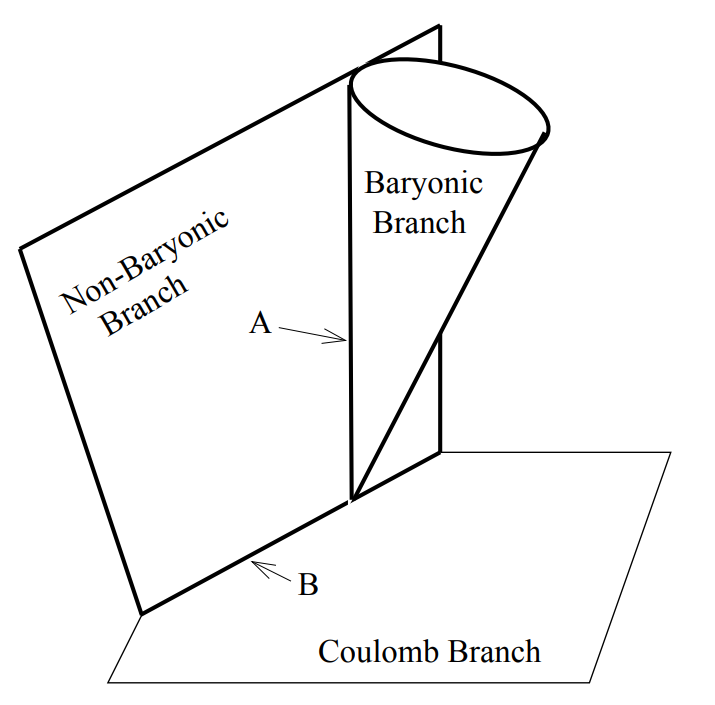
\includegraphics[scale=0.3]{Pictures/classicalmodulispace.png}
            \caption{Map of the classical moduli space of $\mN=2$ $\SU(N_c)$ SQCD with $N_f$ fundamental flavors, from \cite{Argyres_1996}.}
        \end{figure}

\section{Quantum moduli space}\label{secquantummodulispaceSU}

    There are no quantum corrections to the baryonic and non baryonic branches, only the coulomb branch receives quantum corrections. However, the baryonic and non-baryonic roots, that is the submanifolds where they intersect the Coulomb branch, can be modified. The mixed non-baryonic branch will retain its classical product structure.

    We concentrate on the asymptotically free and finite theories with $N_f\leq2N_c$.

    \subsection{Non-baryonic roots}

        The roots are the IR free or finite $\SU(r)\times\U(1)^{N_c-r}$ SQCD with $N_f$ hypermultiplets in the fundamental representation and charged under one of the $\U(1)$ factor.At special points along these manifolds, the SW curve shows that $N_r-r-1$ additional massless singlet hypermultiplets arise, each one charged under one of the remaining $\U(1)$ factors. There are $2N_c-N_f$ such vacua, related by the broken $\Z_{2N_f-N_c}$ non-anomalous $R$-symmetry acting on the Coulomb branch.

    \subsection{Baryonic root}

        For $N_f\leq 2N_c$ (UV free theory), $\U(1)_R$ symmetry of the classical theory is broken down by anomalies to a discrete $\Z_{2N_c-N_f}$ symmetry, which acts on the VEV of $\phi$ by a phase. By the non-renormalization theorem, the fact that the baryonic root is a single point cannot be modified at quantum level. The most general VEV for $\phi$ is therefore a single point invariant under $\Z_{2N_c-N_f}$ thus its coordinates on the Coulomb branch are
        \begin{equation}
            \Phi_{\text{bb}}=\text{diag}(\underbrace{0,\dots,0}_{N_f-N_c},\phi\omega,\phi\omega^2,\dots,\phi\omega^{2N_c-N_f})\label{eq:quantumbaryonicroot}
        \end{equation}
        with $\omega\equiv\zeta_{2N_c-N_f}=e^{i\frac{2\pi}{2N_c-N_f}}$ for some value of $\phi\in\C$. There is only one such point, up to overall renormalization, since the components of $\phi$ are identified up tu permutations. Classically, $\phi=0$. The gauge group is thus unbroken to $\SU(N_f-N_c)\times\U(1)^{2N_c-N_f}$, which is IR free. There are $N_f$ fundamental hypermultiplets. 
        
        Since this theory is IR free, the gauge symmetry is expected to survive at quantum level. However, quantum effects could change this effective theory by bringing additional light degrees of freedom. In particular, there are many point on the submanifold \eqref{eq:quantumbaryonicroot} where monopoles singlets charged under the $\U(1)$ factors become massless. One can show that this theory does not have any purely hypermultiplet Higgs branch, like the baryonic one, unless there is at least one singlet charged under each $\U(1)$ factor. Does such a point exists in \eqref{eq:quantumbaryonicroot}? Using the exact solution, one can show that such a point exist, with precisely $2N_c-N_f$ massless hypermultiplets charged under the $\U(1)$ factors. This singles out the point $\phi=\Lambda$ in the submanifold \eqref{eq:quantumbaryonicroot}.

        Substituting this in the SW curve \eqref{eq:SWcurveCoulombbranch}, we get the singular form
        \begin{equation}
            y^2=x^{2(N_f-N_c)}(x^{2N_c-N_f}+\Lambda^{2N_c-N_f})^2.
        \end{equation}
        The $x^{2(N_f-N_c)}$ factor corresponds to the unbroken $\SU(N_f-N_c)$ gauge group. The remaining $2(2N_c-N_f)$ branch points show up in coincident pairs, located at $x_k=\Lambda\omega^{k-\frac{1}{2}}$ with $k=1,\dots,2N_c-N_f$, corresponding to the $2N_c-N_f$ mutually local massless hypermultiplets.

    \subsection{Summary}

        The roots of the non-baryonic branches are where the gauge symmetry is enhanced to $\SU(r)\times\U(1)^{N_c-r}$ with $N_f$ flavors, just as in the classical analysis.

        The root of the baryonic branch has an unbroken gauge symmetry $\SU(N_f-N_c)\times\U(1)^{2N_c-N_f}$ with $N_f$ flavors in some singlets.

        These are all non-asymptotically-free theories, and so are weakly coupled in the IR. This information can be used to precisely locate the roots, using the exact solution of Coulomb branch.


\part{$A_1$ singularity}

\section{The quiver gauge theory}

    \subsection{Content and lagrangian}

        We consider $N$ D$3$-branes at on an $A_1$ singularity, i.e. probing the transverse space $\C\times\C/\Z_2$ and located at the singularity. To find the low-energy theory, we proceed to the usual orbifold projection for $\Gamma=\Z_2$. $\Gamma$ acts on $\C^n$ through the regular representation as $\rho^N_{\text{reg}}=(\rho_0\oplus\rho_1)^N=\rho^N_0\oplus\rho^N_1$, so $N=n/2$ and the projected gauge group is $G=\U(N)\times\U(N)$. Since $\Gamma\subset\SU(2)$, the theory automatically anomaly free (because chiral). The orbifold group acts as
        \begin{equation}
            \begin{bmatrix}
                1 & 0 & 0 \\
                0 & \zeta_2 & 0 \\
                0 & 0 & \zeta_2
            \end{bmatrix}
        \end{equation}
        on the transverse space. The invariant configurations read
        \begin{align}
            &X^{0,1}_{00}\in(\boldsymbol{N_0},\bar{\boldsymbol{N_0}}),\qquad X^{0,1}_{11}\in(\boldsymbol{N_1},\bar{\boldsymbol{N_1}}),\qquad (\equiv\Phi,\tilde{\Phi})\\
            &X^{2,3}_{01}\in(\boldsymbol{N_1},\bar{\boldsymbol{N_0}}),\qquad X^{2,3}_{10}\in(\boldsymbol{N_0},\bar{\boldsymbol{N_1}}),\qquad (\equiv A_1,B_1)\\
            &X^{4,5}_{01}\in(\boldsymbol{N_1},\bar{\boldsymbol{N_0}}),\qquad X^{4,5}_{10}\in(\boldsymbol{N_0},\bar{\boldsymbol{N_1}}),\qquad (\equiv A_2,B_2)
        \end{align}
        where each $X^m_{ij}$ is an $N_i\times N_j$ block. In conclusion, the low-energy theory is a four-dimensional $\mN=2$ gauge theory with $\U(N)\times\U(N)$ gauge group and $2$ bi-fundamental hypermultiplets and the field content is the following:
        \begin{itemize}
            \item $A_1,A_2$ transforming in the $(\boldsymbol{N_1},\bar{\boldsymbol{N_0}})$ are the two complex scalars of the first hypermultiplet. They are in $\mathfrak{u}(N)$.
            \item $B_1,B_2$ transforming in the $(\boldsymbol{N_0},\bar{\boldsymbol{N_1}})$ are the two complex scalars of the second hypermultiplet. They are in $\mathfrak{u}(N)$.
            \item $\Phi,\tilde{\Phi}$ are transforming in the $(\boldsymbol{N_0},\bar{\boldsymbol{N_0}})$ and $(\boldsymbol{N_1},\bar{\boldsymbol{N_1}})$ respectively, i.e. in the adjoint of each factor of the gauge group. They are part of the the $\U(N)\times\U(N)$ vector multiplet.
        \end{itemize}

        The quiver of the theory is given by
        \begin{center}
            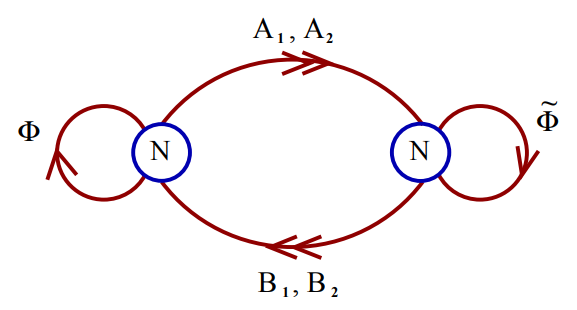
\includegraphics[scale=0.35]{Pictures/A1quiver.png}
        \end{center}
        and has adjacency matrix
        \begin{equation}
            \begin{bmatrix}
                1 & 2 \\
                2 & 1
            \end{bmatrix}.  
        \end{equation}

        The lagrangian can be obtained from $D=4$ $\mN=4$ pure SYM with $\U(2N)$ gauge group by substituting the invariant configurations that we found. The $\mN=4$ vector multiplet can written in terms $\mN=1$ fields as one vector multiplet $V$ and three chiral multiplets $\Phi^A$, $A=1,2,3$, all fields in the adjoint of $\U(2N)$. The invariant configuration are
        \begin{equation}
            \Phi^1=
            \begin{bmatrix}
                \Phi & 0 \\
                0 & \tilde{\Phi}
            \end{bmatrix},\qquad
            \Phi^2=
            \begin{bmatrix}
                0 & A_1 \\
                B_2 & 0
            \end{bmatrix},\qquad
            \Phi^3=
            \begin{bmatrix}
                0 & A_2 \\
                B_1 & 0
            \end{bmatrix}.\label{eqinvconf}
        \end{equation}
        The gauge transformation of the fields $A_i,B_i\Phi,\tilde{\Phi}$ coming from the transformation of $\Phi^1,\Phi^2,\Phi^3$ are indeed what we found before. The superpotenntial is obtained from the the superpotenntial of $\mN=2$ SYM ($\Phi^1[\Phi^2,\Phi^3]$) by substituting \eqref{eqinvconf}:
        \begin{equation}
            W=(B_1\Phi A_1-B_2\Phi A_2)-(A_1\tilde{\Phi}B_1-A_2\tilde{\Phi}B_2).
        \end{equation}

        We are interested by the superconformal theory with gauge group $\SU(N+M)\times\SU(N)$. The latter can be obtained from our original theory through the following steps:
        \begin{alignat}{2}
            \U(N)\times\U(N)&\to \SU(N+M)\times\SU(N+M)\qquad&&\text{redefining $N$}\\
            &\to \U(N+M)\times\U(N)\times\U(1)^M\qquad&&\text{Higgsing: we taking $M$ VEV's $\abs{z_0}/2\pi\alpha'$ in $\tilde{\Phi}$}\\
            &\to \SU(N+M)\times\SU(N)\qquad&&\text{low-energy limit}.\label{eq:theorymanip}
        \end{alignat}


    \subsection{Classical moduli space}

        The F-term equations are
        \begin{equation}
            F:
            \begin{cases}
                \Phi A_i-A_i\tilde{\Phi} = 0\\
                B_i\Phi-\tilde{\Phi}B_i = 0\\
                A_1B_1-A_2B_2 = 0\\
                B_1A_1-B_2A_2 = 0
            \end{cases}
        \end{equation}
        In total, there are six different fields, whiwh are all matrices in $\u(N)$, meaning that in total their are $6N^2/2=3N^2$ independent complex parameters. The moduli space is therefore a variety embedded in $\C^{3N^2}$, defined by $\M=Z(F)/G_\C$. Its cooridnate ring is $K[\M]=K[Z(F)]^{G_\C}$ and we must find a generating set of this polynomial ring, i.e. a basis of invariant polynomials. We find the six following coordinates:
        \begin{align}
            \vp_{ij} &= \tr (A_i B_j),\\
            \vp &= \tr(\Phi),
            \tilde{\vp} &= \tr(\tilde{\Phi}).
        \end{align}

        \underline{Coulomb branch:} the fields $\Phi,\tilde{\Phi}$ can be diagonalized by a gauge transformation, leaving $2N$ independant complex parameters. The gauge group breaks to $(\U(1)^{N}\times S_N)\times(\U(1)^{N}\times S_n)=\U(1)^{2N}/(S_N\times S_N)$ and the geometry is
        \begin{equation}
            \M^V_{\text{cl.}} = \frac{\C^N}{S_N}\times\frac{\C^N}{S_N},
        \end{equation}
        which corresponds to the displacement of two types of fractional branes D$3$-branes, each associated to one gauge factor, along the singularity line. The Coulomb branch recieves corrections at the quantum level, this will be discussed later on. The exact quantum-corrected metric is calculable thanks to Seiberg-Witten theory\cite{Witten_1997}.


        \underline{Higgs branch:} it is parametrized by $4N$ complex parameters, which are the VEV's of $A_i,B_i$. These VEV's result in the Higgsing of the quiver to a subgroup of the diagonal $\U(N)$ gauge group and the theory has accidental $\mN=4$ suersymmetry in the IR. Its geometry is
        \begin{equation}
            \M^H_{\text{cl.}} = \frac{(\C\times\C^2/\Z_2)^N}{S_N}.
        \end{equation}
        Because of $\mN=2$ supersymmetry, the Higgs is a Kähler manifold and its metric is classicaly exact, meaning that it is protected against quantum corrections.

        \underline{Mixed branches:} are also present.

\section{Type IIB supergravity dual solution}

    The initial observation is that the large $N$ limit of certain conformal field theories in various dimensions include in their Hilbert space a sector describing supergravity on the product of anti-de-Sitter spacetimes, spheres and other compact manifolds \cite{Maldacena:1997re}. This was shown by taking some branes in the full M/string theory and then taking a low energy limit where the field theory on the brane decouples from the bulk. In this limit, we can still trust the near horizon geometry for large $N$. The enhanced supersymmetries of the near horizon geometry correspond to the extra supersymmetry generators present in the superconformal group (as opposed to just the super-Poincaré group). The 't Hooft limit of $\mN = 4$ SYM at the conformal point is shown to contain strings: they are IIB strings. It was the conjectured that compactifications of M/string theory on various anti-de-Sitter spacetimes is dual to various conformal field theories.

    Very soon after that, a specific correpsondence between $4d$ $\mN=0,1,2$ SCFT and Type IIB string theory on various orbifolds of $AdS_5\times S^5$ was argued in \cite{silervstein1998}. In particular, in the large $N$ and large 't Hooft coupling limit, the low energy superconformal sector of our $\U(N)\times\U(N)$ theory can be described by its Type IIB supergravity dual. The full Higgs branch is dual to a familly of supergravity solutions corresponding to D$3$-branes at arbitrary positions on the $6$-dismensional transverse space:
    \begin{align}
        ds^2 &= Z^{-1/2}\eta_{\mu\nu}\d x^\mu\d x^\nu+Z^{1/2}\delta_{mn}\d x^m\d x^n\\
        g_s F_5 &= (1+\star)\d\text{vol}_{3,1}\wedge\d Z^{-1}
    \end{align}
    where $\mu\nu,0,\dots,3$ denotes the brane worldvolume coordinates and $m,n=4,\dots,9$ the transverse coordinates. The transverse space is a $\Z_2$-orbifold so we have the identification $\textbf{x}\sim\tilde{\textbf{x}}$ with
    \begin{align*}
        \textbf{x} &\equiv (x^4,x^5,x^6,x^7,x^8,x^9),\\
        \tilde{\textbf{x}} &\equiv (x^4,x^5,-x^6,-x^7,-x^8,-x^9)
    \end{align*}
    $Z$ is the harmonic function
    \begin{equation}
        Z(x^4,\dots,x^9)=4\pi g_s(\alpha')^2\sum^N_{j=1}\left( \frac{1}{\abs{\textbf{x}-\textbf{x}_j}^4}+\frac{1}{\abs{\textbf{x}-\tilde{\textbf{x}}_j}^4} \right)
    \end{equation}
    containing the D$3$-branes and their image. We see that the total $5$-form flux on $S^5/\Z_2$ at infinity is $N$. The relations between the field theory and the supergravity solution is
    \begin{itemize}
        \item the relation between the parameters $x_j$ (positions of the branes on the orbifold) and the field theory moduli is $x_j=2\pi\alpha'\phi_j$, where $\phi_j$ is the eigenvalue of the VEV of some field
        \item the coordinates $\vp$ and $\tilde{\vp}$ are mapped to $x^4+i x^5$
        \item the coordinates are mapped to $\vp_{ij}$ to the algebraic coordinates $z_{ij}$ on $\C^2/\Z_2$, such that $z_{12}z_{21}=z^2_{11}$ and $z_{22}=z_{11}$.
        \item the supergravity axio-dilaton $\tau=C_0+ie^{-\Phi}=C_0+i/g_s$ is constant, as D$3$-branes are not coupled to it. It is related to the field theory gauge coupling and theta angles by
        \begin{equation}
            \tau = \tau_1+\tau_2, \qquad \tau_j = \frac{\theta_j}{2\pi}+\frac{4\pi i}{g^2_j}.
        \end{equation}
    \end{itemize}
    We take $\tau=i/g_s$.

    The Coumob branch of our theory is described by fractional D$3$-branes alongs the orbifold singularity. In this case, the supergravity solutions include non-travial profile for the twisted field fluxes. Indeed, fraction D$3$-branes source magnetically the twisted scalar $c$ and, by supersymmetry, they also soure its NS-NS partner, the twisted scalar $b$. This can be understood recalling that fractional D$3$-branes are equivalent to D$5$-branes wrapped around the exceptional $2$-cycle $\mathcal{C}$ which lives at the orbifold ingularity. The twisted scalars are simply the reduction of the R-Rand NS-NS 2-form potentials $C_2$ and $B_2$, on $\mathcal{C}$:
    \begin{equation}
        c = \frac{1}{4\pi^2\alpha'}\int_\mathcal{C}C_2,\qquad b = \frac{1}{4\pi^2\alpha'}\int_\mathcal{C}B_2.
    \end{equation}
    They can be organized in a single complex scalar as
    \begin{equation}
        \gamma=c+\tau b
    \end{equation}
    where took $\tau=i/g_s$.

    For $N$ fractional branes at $z_1,\dots,z_N$ and $N$ anti-fractional\footnote{Branes wrapped around $\mathcal{C}$ with the opposite orientation.} branes at $\bar{z}_1,\dots,\bar{z}_N$, we have
    \begin{equation}
        \gamma=\frac{i}{\pi}\left[ \sum^N_{j=1}\log(z-z_j)-\sum^N_{j=1}\log(z-\bar{z}_j) \right]+\gamma^{(0)}.\label{eq:gammasol}
    \end{equation}
    The $\SU(N+M)\times\SU(M)$ quiver gauge theory obtained in \eqref{eq:theorymanip} corresponds, in the dual picture, to placing $M$ anti-fractional branes at the roots $\tilde{z}^M_j=-z^M_0$ while theo other $N$ anti-fractional branes and $N+M$ fractional branes sit at the origin. This configuration gives us
    \begin{equation}
        \gamma(z)=\frac{i}{\pi}\log\frac{z^M}{z^M+z^M_0}+\gamma^{(0)}.
    \end{equation}
    For simplicity, we set the point value orbifold $\gamma^{(0)}=i/2g_s$ so that, in the UV, $\tau_1=\tau_2=i/g_s$. In the large $M$ limit, \eqref{eq:gammasol} becomes
    \begin{equation}
        \gamma=
        \begin{cases}
            i\frac{M}{\pi}\log\frac{z}{z_0}+\frac{i}{2g_s}\ = i\frac{M}{\pi}\log\frac{z}{z_1},\qquad \text{ if } \abs{z}<\abs{z_0}\\
            \gamma^{(0)},\hspace{3.8cm}\qquad \text{ if } \abs{z}>\abs{z_0}
        \end{cases}\label{eq:flux1}
    \end{equation}
    with $z_1\equiv e^{i\frac{\pi}{M}\gamma^{(0)}}=e^{-\frac{\pi}{2g_sM}}$.

    For $r<\rho_0=\abs{z_0}$, the gauge invariant D$3$-brane Maxwell charge carried by the fluxes of the solution is
    \begin{equation}
        -\frac{1}{(2\pi^2\alpha')^2}\int F_5=N+\frac{g_sM^2}{\pi}\log\frac{r}{\rho_1}\label{eq:flux2}
    \end{equation}
    where $\rho_1=\abs{z_1}$.

    \begin{mybox}
        Below the cutoff $\rho_0$, the solution enjoys logarithmically varying $B$-field and $5$-form flux. This similarity with the Klebanov-Tseytlin solution suggests the dual theory might enjoy a cascading RG flow with subsequent infinite coupling transition reducing the rank of the infinitely-coupled non-abelian gauge group by $2M$ at scales $\rho_k=e^{-\frac{(2k-1)\pi}{2g_sM}}\rho_0$, with $k=1,\dots,l$ and $l=\lfloor N/M \rfloor$.
    \end{mybox}

\section{Enhançon mehcanism, quantum Coulomb branch and SW curves}

    There is another problem of the supergraity solution that one has to deal with. This problem always arises in supergravity solutions dual to non-conformal sueprsymmetric gauge theories with eight supercharges: by analyzing the explicit form of the warp factor, one can show that the $10$-dimensional metric obtained using \eqref{eq:gammasol} possesses, besides the orbifold singularity, an unphysical repulsive region near the origin. An enhançon-like mechanism is therefore expected, in order to excise the unphysical region, thus rendering back a repulsion-free solution.

    While the Higgs branch is classicaly exact, it is not the case of the Coulomb branch. At the classical level, the VEV's of the adjoint scalars correspond to the position of the fraction and anti-fractional branes. In the quantum theory, this identification cannot survive because, while the VEV's are still unconstrained, the position of the branes become constrained.
        
    Because of supersymmetry, one expects that, in the large $N$ limit, the quantum corrections and the consequent constraints on $z_j$ and $\tilde{z}_j$ are bound to a non-negative $5$-form flux for allowed configurations on the quantum moduli space, at least whenever the supergravity approximation is valid. This property is the core of the enhançon mechanism.

    Let us discuss the SW curves of the $\SU(N+M)\times\SU(N)$ theory. Since the second gauge group is not asymptitcally free, one should embed theory into the $\SU(N+M)\times\SU(N+M)$ superconformal one, properly Higgsed, as explained before. We define the complex coordinate
    \begin{equation}
        u=i\frac{x^6+ix^{10}}{2\pi R_{10}}
    \end{equation}
    which parametrizes the M-theory torus defined by the identification $u\sim u+\tau$. The complex structure $\tau$ is identified with the Type IIB axio-dilaton. Retricting ourselves to the case of equal gauge couplings $\tau_1=\tau_2=\tau/2$, the Sw curve for the conformal theory reads
    \begin{equation}
        \frac{R(v)}{S(v)}=g(u|\tau)
    \end{equation}
    where $g(u|\tau)$ is a combination of quasi-modular Jacobi $\theta$-functions
    \begin{equation}
        R(v)=\prod^{N+M}_{a=1}(v-\phi_a),\qquad S(v)=\prod^{N+M}_{a=1}(v-\tilde{\phi}_a)
    \end{equation}
    are polynomials of degree $N+M$ whose zeros $\phi_a$ and $\tilde{\phi}_a$ are the eigenvalues of the VEV's of the adjoint scalar fields of the first and second gauge group respectively. 
    
    Comparing the SW curve at the origin, we can see that the dynamically generated scale is $\Lambda=e^{\frac{\pi i \tau}{2M}}z_0$. One can check that:
    \begin{itemize}
        \item \underline{for $\abs{v}>\abs{z_0}$:} the quantum theory is conformal with equal gauge couplings.
        \item \underline{for $\abs{\Lambda}<\abs{v}<\abs{z_0}$:} the two couplings are running with opposite $\beta$-functions:
        \begin{equation}
            \beta_{1,2} = \pm 2M\label{eq:betafct}.
        \end{equation}
        \item \underline{at $\abs{v}=\abs{\Lambda}$:} the gauge group is effectively broken by instantons as
        \begin{equation}
            \SU(N+M)\times\SU(N)\times\U(1)^M\to\SU(N)\times\SU(N)\times\U(1)^{2M},
        \end{equation}
        the residual gauge group being conformal up to an IR free abelian sector.
        \item \underline{for $\abs{v}<\abs{\Lambda}$:} the gauge couplings are constant with $8\pi^2/g^2_{s,1}=0$ and $8\pi^2/g^2_{s,2}=2\pi/g_s$.
    \end{itemize}

    \begin{figure}[H]
        \centering
        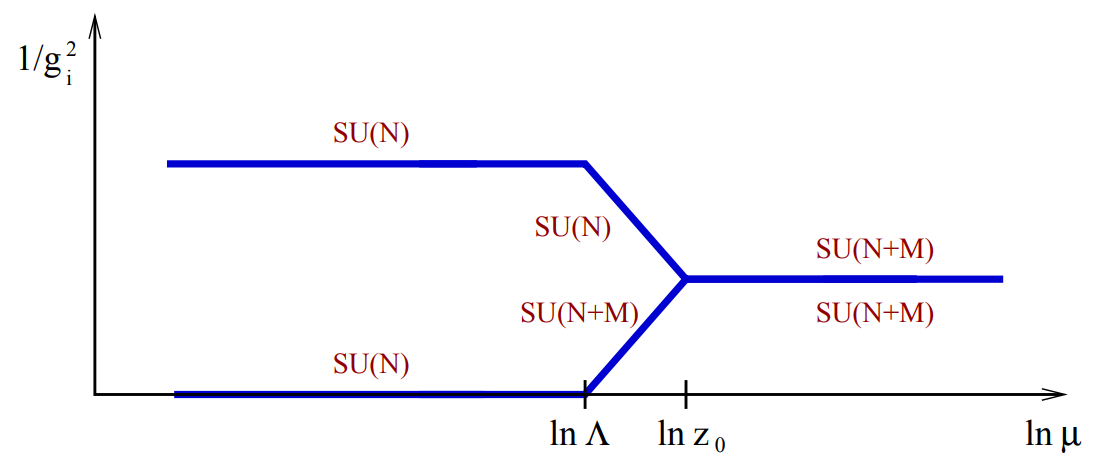
\includegraphics[scale=0.3]{Pictures/RGflow.png}
        \caption{RG flow of the theory at the enhançon vacuum (origin of the moduli space). The low-energy theory below $\Lambda$ is a peculiar one, with one formally diverging coupling.}
    \end{figure}

    Further information is gained by the computation of the branch points of the SW curve. the first set is located at
    \begin{equation}
        u=\frac{\tau}{2},\frac{\tau+1}{2}:\qquad v=v^\pm_h=z_0e^{\frac{2\pi i h}{M}}\left[ 1\pm \frac{2}{M}\left( \frac{\Lambda}{z_0} \right)^M \right],\qquad h=1,\dots,M
    \end{equation}
    and are almost double branch points, which corresponds to the $M$ anti-fractional branes located near $\abs{z_0}$, corresponding to the VEV's of $\tilde{\Phi}$ we used to Higgs the conformal theory. The second set is located at
    \begin{equation}
        u=0,\frac{1}{2}:\qquad v=v_k=2^{\frac{1}{M}}e^{\frac{\pi i k}{M}}\Lambda,\qquad k=1,\dots,2M.
    \end{equation}
    These branch points correspond to $M$ fractional branes melted into en enhançon ring at scale $\Lambda$.

    Probe fractional branes can be studied on this background by means of the SW curve of the $\SU(N+M+1)\times\SU(N+M+1)$ theory, where the VEV's of $\Phi$ and $\tilde{\Phi}$ now have an extra eigen value that we denote $\phi$ and $\tilde{\phi}$. We find that the branch points corresponding corresponding to the eigenvalue $\phi$ (the fraction brane) can freely move outside the enhancon ring, but as they approach the enhançon ring and $\phi$ goes to zero, the two branch points split and melt into the anhançon ring. The two branch points corresponding to the eigenvalue $\tilde{\phi}$ (the anti-fractional brane) can instead penetrate the enhançon ring.Whe this happens, they unchain two branch points from the ring which follow them inside: an anti-fractional brane eats a melted fractional brane from the ring, thus forming a regular brane free to move everywhere.

    We conclude that, no matter the value of $N$, the fluxes in \eqref{eq:flux1} and \eqref{eq:flux2} do describe the physics of the $\SU(N+M)\times\SU(N)$ theory at the origin of its moduli space, provided that they are excised at radius $\rho_1=\abs{\Lambda}$ by an enhançon mechanism. The solution should also be cut off at radius $\abs{z_0}$, or completed with $M$ fractional branes, providing a conformal $AdS_5$ UV completion. The warp factors then needs to be recomputed in the presence of the correct brane configuration.

    \begin{mybox}
        The $10$-dimensional metric possesses an unphysical repulsive region around the origin. It is expected that an enhancon-like mehcanism will excise this unphyiscal region. This indeed what happens: using the SW curve technology, one finds that, in the quantum theory, fractional branes melt into an enhançon ring at scale $\Lambda$. Anti-fractional branes can penetrate this ring by eating a fractional brane on the way, thus forming a regular brane that is free to move everywhere.
    \end{mybox}

    Notice that the supergravity solution \eqref{eq:flux1} and \eqref{eq:flux2} does not seem to have any pathology below $\rho_1$, at least down to a scale of order $e^{-\frac{\pi N}{g_s M^2}}\rho_1$, where the $5$-form flux \eqref{eq:flux2} vanishes and the problematic region starts. The question arises whether there is any field theory interpration for such a solution, suitbaly excised only at radius
    \begin{equation}
        \rho_{\text{min}}=\rho_{l+1}\equiv e^{-\frac{\pi l}{g_s M}}\rho_1
    \end{equation}
    with $l=\lfloor N/M\rfloor$, the smallest infinite coupling scale outside the region of nagative D$3$ brane charge. Based on results about $\mN=2$ SQCD, it was proposed that there exists a field theory vacua, not at the origin of hte Coulomb branch, which display csacading bahavior. Theyare dual to the supergravity solution \eqref{eq:flux1} and \eqref{eq:flux2}, valid well below the first infinite coupling radius $\rho_1$ down to smoe much lower scale, at most until the so-called true anhançon scale $\rho_{\text{min}}$ where the twisted fields are excised.
        
\section{RG flow}

    The beta function of both $\SU(N)$ factors vanish. The duagonal $\U(1)$ is decoupled and the anti-diagonal $\U(1)$ becomes free in the IR and gives rise to a global symmetry, the baryonic symmetry $\U(1)_B$.

\section{Cascading vacuum}

    The perturbative RG flow of the $\SU(N+M)\times\SU(N)$ theory described is given by \eqref{eq:betafct}. It such that the largest group goes to strong coupling at a scale $\Lambda$ while the smallest group goes to a fixed, lower coupling. The dual supergravity solution suggests that, in the dual vacuum, a mechanism effectively reduces the gauge group as
    \begin{equation}
        \SU(N+M)\times\SU(N)\to\SU(N-M)\times\SU(N)\label{eq:gaugegroupereduction}
    \end{equation}
    below $\Lambda$, plus possible $\U(1)$ factors. 
    
    This statement is supported by a computation of Page charges in supergravity. We find
    \begin{align}
        Q^{\text{Page}}_{\text{D3}}(r) &= -\frac{1}{4\pi^2\alpha'}\int (F_5+B_2\wedge F_3))=N+M\left\lfloor\frac{g_sM}{\pi}\log\frac{r}{\rho_0}\right\rfloor,\\
        Q^{\text{Page}}_{\text{D5}}(r) &= -\frac{1}{4\pi^2\alpha'}\int F_3=2M
    \end{align}
    with $\rho\equiv\abs{z}$. Positivity of the charges implies
    \begin{equation}
        r>(e^{-\frac{\pi}{g_sM}})^{\frac{N}{M}}\rho_0.
    \end{equation}
    This shows that the reduction of the gauge group \eqref{eq:gaugegroupereduction} does not only happens at the first strong coupling scale $\Lambda$ but actually each generalized enhançon, occuring at scales
    \begin{equation}
        \rho_k=\Lambda_k\equiv e^{-\frac{\pi(k-1)}{g_sM}}\Lambda_1 = e^{-\frac{\pi(2k+1)}{2g_sM}}\rho_0, \qquad k=1,\dots,l
    \end{equation}
    where $N=lM+p$, i.e. $l=\lfloor N/M\rfloor$ and $\Lambda_1\equiv\Lambda$. At each step, the rank of the biggest group decreases by $2M$. There are therefore $l$ steps:
    \begin{center}
        $\SU(N+M)\times\SU(N)$\\
        $\downarrow$\\
        $\SU(N-M)\times\SU(N)$\\
        $\downarrow$\\
        $\SU(N-M)\times\SU(N-2M)$\\
        $\downarrow$\\
        $\SU(N-3M)\times\SU(N-2M)$\\
        $\vdots$\\
        $\SU(M+p)\times\SU(N-(l-1)M)$\\
        $\downarrow$\\
        $\SU(M+p)\times\SU(p)$\\
    \end{center}
    %where, by convention, we wrote the bigger group first in the product, i.e. there is a permutation at each new line. 
    Note that $\lfloor N/M\rfloor$ or $\lfloor(N+M)/M\rfloor$ is even so, in the end, the gauge group is always $\SU(M+p)\times\SU(p)$, upon a possible parmutation of the factors.

    There are two steps that on has to add to this to obtain the complete evolution of the gauge group for all scales: the Higgsing step at scale $\abs{z_0}$ that allows us introduce a difference in the gauge group ranks and the last step, at $\Lambda_{l+1}=\Lambda_{\text{min}}=e^{-\frac{\pi l}{g_s M}}\Lambda_1$. Below $\Lambda_{l+1}$, there is a true anhançon ring with $M$ tensionless fractional branes, and the non-abelian factors in the gauge group reduce according to
    \begin{equation}
        \SU(M+p)\times\SU(p)\to\SU(p)\times\SU(p),
    \end{equation}
    with one infinite gauge coupling. Twisted fields have to be excised so as to avoid negative D$3$-brane charge in the interior region.

    

    \subsection{One cascade step: $\mN=2$ SQCD}

        To devlop an intuition of the coupling dynamics, we can start by focussing on the first such generalized enhançon, which accurs at scale $\Lambda_1$. This will be a prototype for each generalized enhançon. Moreover, for simplicity, we can consider a corner of the parameter space of the gauge theory: the limit $Ng^2_{\text{min}}\to0$. In this limit, the gauge dynamics of the second factor in the gauge group decouples and effectively becomes a global symmetry. Consequently, the theory around $\Lambda_1$ is $\SU(N+M)$ SQCD with $2N$ flavors. The VEV's for the smaller group adjoint-scalar effectively behaves as masses for the larger group hypermultiplets. In this case, we are out of the supergravity approximation but it will still give some good insights.

        We discussed the form of the quantum baryonic root in \ref{secquantummodulispaceSU}. We found that it preserves the same $\Z_{2N_c-N_f}=\Z_{2M}$ R-symmetry as the supergravity solution we are discussing. Moreover, its low energy effective theory possesses an $\SU(N_f-N_c)=\SU(N-M)$ gauge symmetry. This precisely matches the numerology of the cascading interpretation. Hence, iterating the same procedure at the subsequent generalized enhançon $\Lambda_k$ (where the higher rank gauge group coupling diverges), it is natural to propose the supergravity solutions in \todo{to complete} (excised only down at the true enhançon $\rho_{\text{min}}$) to be dual to a cascading $\SU(N+M)\times\SU(N)$ quiver gauge theory at subsequent baryonic roots of the strongly coupled gauge groups.

        \begin{mybox}
            The non-perturbative dynamics at the baryonic roots possesses the same R-symmetry as the dual supergravity solution. Moreover its low energy effective theory possesses an $\SU(N_f-N_c)=\SU(N-M)$ gauge symmetry, thus matching the numerology of the cascading interpretation. Iterating the same procedure at the subsequent generalized enhançon, it is natural to propose the supergravity solution \eqref{eq:flux1} and \eqref{eq:flux2} (excised only down at the true enhançon $\rho_{\text{min}}$) to be dual to a cascading $\SU(N+M)\times\SU(N)$ quiver gauge theory at subsequent baryonic roots of the strongly coupled gauge groups.
        \end{mybox}

    \subsection{Cascading vacuum in the quiver gauge theory}



    \begin{figure}[H]
        \centering
        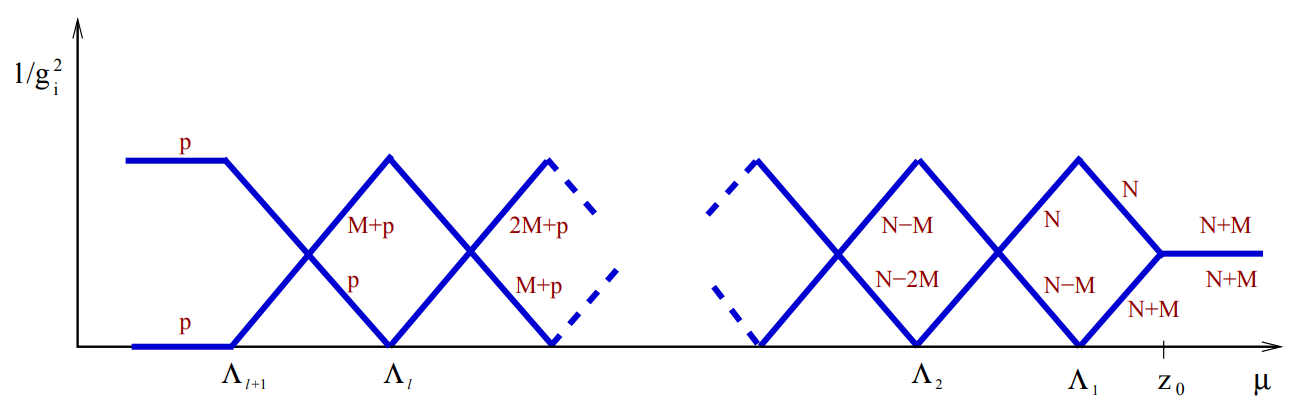
\includegraphics[scale=0.3]{Pictures/RGflowcascade.png}
        \caption{RG flow of the theory at the cascading vacuum, without the $\SU$ factors for the gauge groups, to avoid clutter.}
    \end{figure}



\section{Generalization to $A_n$ singularity}

\part{$\D_4$ singularity}